\documentclass[1p]{elsarticle_modified}
%\bibliographystyle{elsarticle-num}

%\usepackage[colorlinks]{hyperref}
%\usepackage{abbrmath_seonhwa} %\Abb, \Ascr, \Acal ,\Abf, \Afrak
\usepackage{amsfonts}
\usepackage{amssymb}
\usepackage{amsmath}
\usepackage{amsthm}
\usepackage{scalefnt}
\usepackage{amsbsy}
\usepackage{kotex}
\usepackage{caption}
\usepackage{subfig}
\usepackage{color}
\usepackage{graphicx}
\usepackage{xcolor} %% white, black, red, green, blue, cyan, magenta, yellow
\usepackage{float}
\usepackage{setspace}
\usepackage{hyperref}

\usepackage{tikz}
\usetikzlibrary{arrows}

\usepackage{multirow}
\usepackage{array} % fixed length table
\usepackage{hhline}

%%%%%%%%%%%%%%%%%%%%%
\makeatletter
\renewcommand*\env@matrix[1][\arraystretch]{%
	\edef\arraystretch{#1}%
	\hskip -\arraycolsep
	\let\@ifnextchar\new@ifnextchar
	\array{*\c@MaxMatrixCols c}}
\makeatother %https://tex.stackexchange.com/questions/14071/how-can-i-increase-the-line-spacing-in-a-matrix
%%%%%%%%%%%%%%%

\usepackage[normalem]{ulem}

\newcommand{\msout}[1]{\ifmmode\text{\sout{\ensuremath{#1}}}\else\sout{#1}\fi}
%SOURCE: \msout is \stkout macro in https://tex.stackexchange.com/questions/20609/strikeout-in-math-mode

\newcommand{\cancel}[1]{
	\ifmmode
	{\color{red}\msout{#1}}
	\else
	{\color{red}\sout{#1}}
	\fi
}

\newcommand{\add}[1]{
	{\color{blue}\uwave{#1}}
}

\newcommand{\replace}[2]{
	\ifmmode
	{\color{red}\msout{#1}}{\color{blue}\uwave{#2}}
	\else
	{\color{red}\sout{#1}}{\color{blue}\uwave{#2}}
	\fi
}

\newcommand{\Sol}{\mathcal{S}} %segment
\newcommand{\D}{D} %diagram
\newcommand{\A}{\mathcal{A}} %arc


%%%%%%%%%%%%%%%%%%%%%%%%%%%%%5 test

\def\sl{\operatorname{\textup{SL}}(2,\Cbb)}
\def\psl{\operatorname{\textup{PSL}}(2,\Cbb)}
\def\quan{\mkern 1mu \triangleright \mkern 1mu}

\theoremstyle{definition}
\newtheorem{thm}{Theorem}[section]
\newtheorem{prop}[thm]{Proposition}
\newtheorem{lem}[thm]{Lemma}
\newtheorem{ques}[thm]{Question}
\newtheorem{cor}[thm]{Corollary}
\newtheorem{defn}[thm]{Definition}
\newtheorem{exam}[thm]{Example}
\newtheorem{rmk}[thm]{Remark}
\newtheorem{alg}[thm]{Algorithm}

\newcommand{\I}{\sqrt{-1}}
\begin{document}

%\begin{frontmatter}
%
%\title{Boundary parabolic representations of knots up to 8 crossings}
%
%%% Group authors per affiliation:
%\author{Yunhi Cho} 
%\address{Department of Mathematics, University of Seoul, Seoul, Korea}
%\ead{yhcho@uos.ac.kr}
%
%
%\author{Seonhwa Kim} %\fnref{s_kim}}
%\address{Center for Geometry and Physics, Institute for Basic Science, Pohang, 37673, Korea}
%\ead{ryeona17@ibs.re.kr}
%
%\author{Hyuk Kim}
%\address{Department of Mathematical Sciences, Seoul National University, Seoul 08826, Korea}
%\ead{hyukkim@snu.ac.kr}
%
%\author{Seokbeom Yoon}
%\address{Department of Mathematical Sciences, Seoul National University, Seoul, 08826,  Korea}
%\ead{sbyoon15@snu.ac.kr}
%
%\begin{abstract}
%We find all boundary parabolic representation of knots up to 8 crossings.
%
%\end{abstract}
%\begin{keyword}
%    \MSC[2010] 57M25 
%\end{keyword}
%
%\end{frontmatter}

%\linenumbers
%\tableofcontents
%
\newcommand\colored[1]{\textcolor{white}{\rule[-0.35ex]{0.8em}{1.4ex}}\kern-0.8em\color{red} #1}%
%\newcommand\colored[1]{\textcolor{white}{ #1}\kern-2.17ex	\textcolor{white}{ #1}\kern-1.81ex	\textcolor{white}{ #1}\kern-2.15ex\color{red}#1	}

{\Large $\underline{12a_{0326}~(K12a_{0326})}$}

\setlength{\tabcolsep}{10pt}
\renewcommand{\arraystretch}{1.6}
\vspace{1cm}\begin{tabular}{m{100pt}>{\centering\arraybackslash}m{274pt}}
\multirow{5}{120pt}{
	\centering
	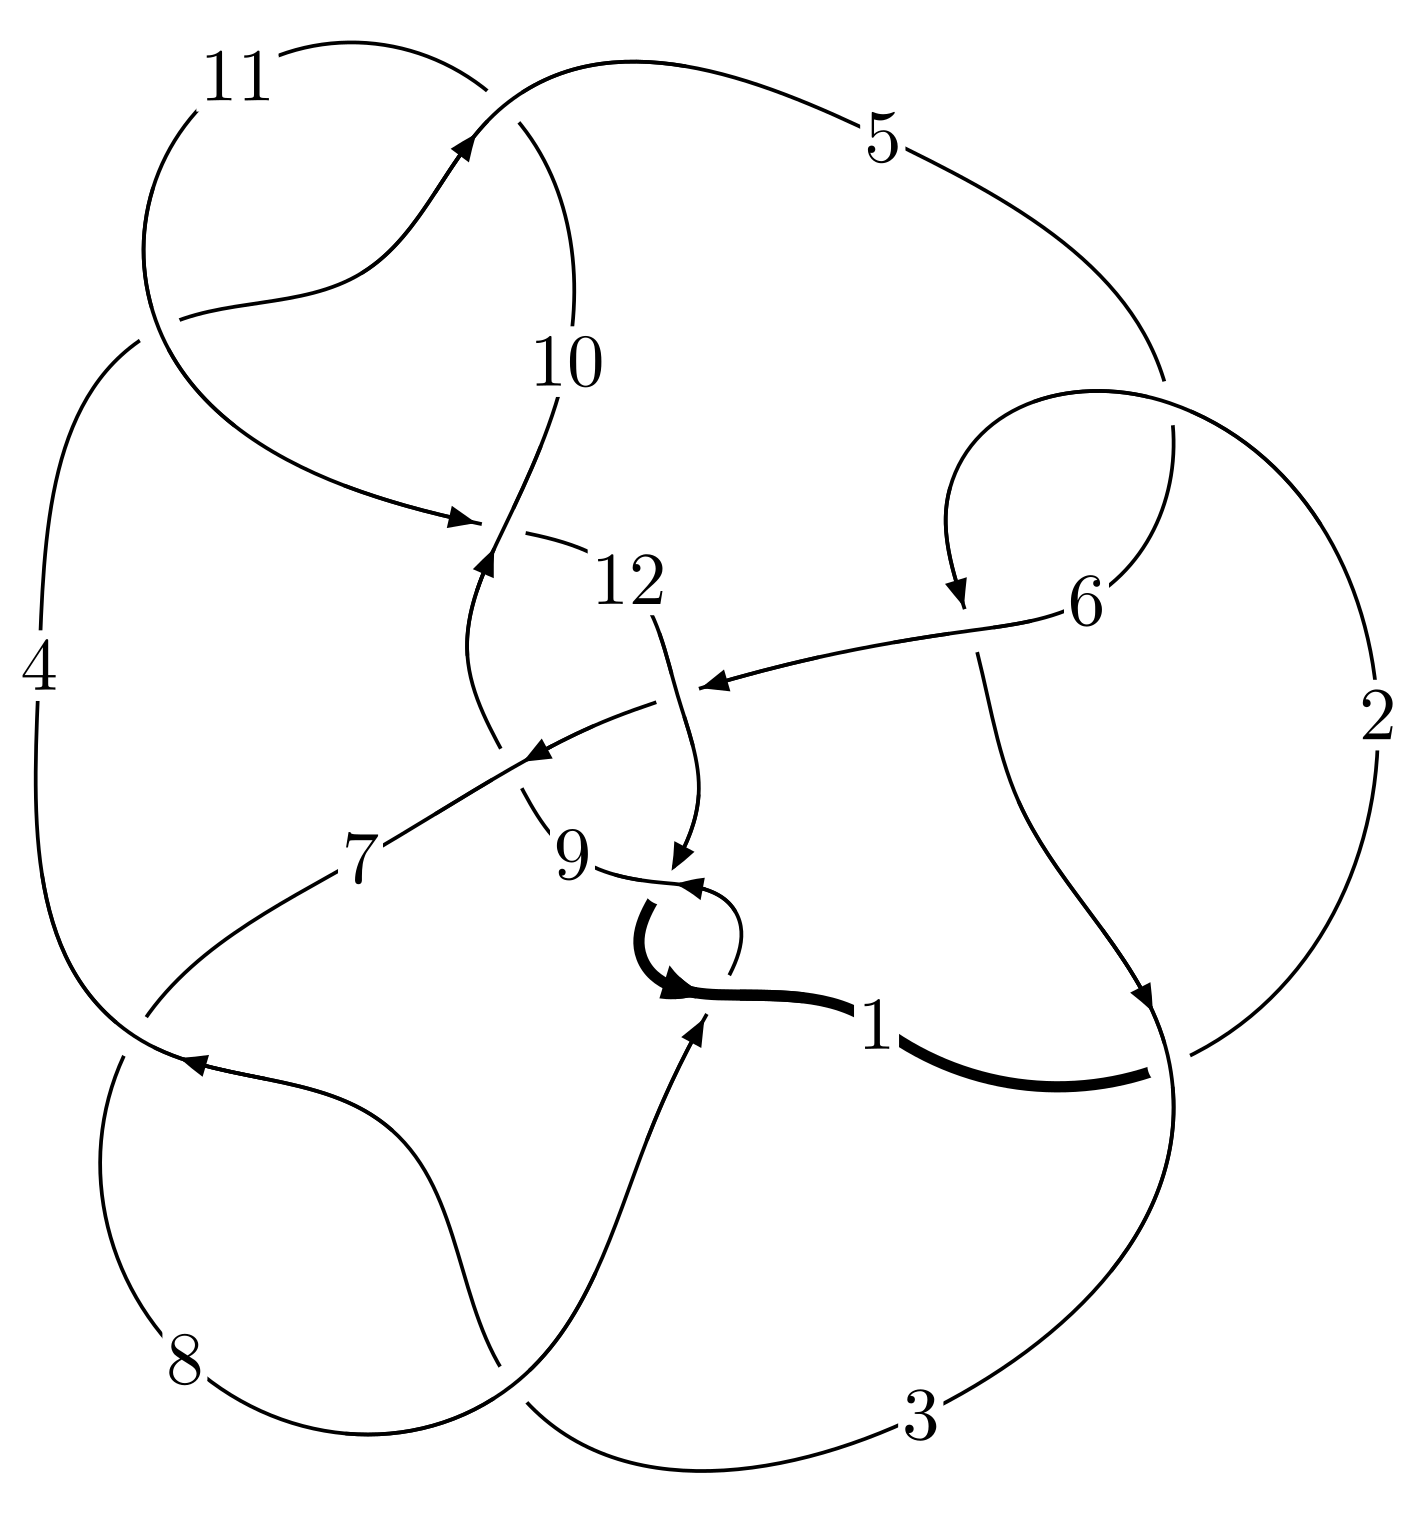
\includegraphics[width=112pt]{../../../GIT/diagram.site/Diagrams/png/1127_12a_0326.png}\\
\ \ \ A knot diagram\footnotemark}&
\allowdisplaybreaks
\textbf{Linearized knot diagam} \\
\cline{2-2}
 &
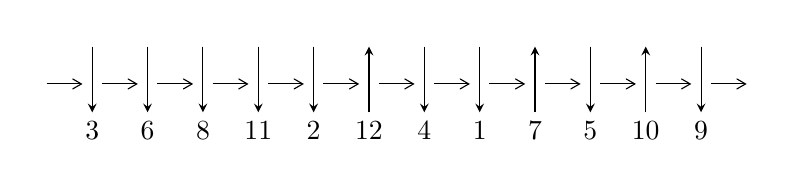
\begin{tikzpicture}[x=20pt, y=17pt]
	% nodes
	\node (C0) at (0, 0) {};
	\node (C1) at (1, 0) {};
	\node (C1U) at (1, +1) {};
	\node (C1D) at (1, -1) {3};

	\node (C2) at (2, 0) {};
	\node (C2U) at (2, +1) {};
	\node (C2D) at (2, -1) {6};

	\node (C3) at (3, 0) {};
	\node (C3U) at (3, +1) {};
	\node (C3D) at (3, -1) {8};

	\node (C4) at (4, 0) {};
	\node (C4U) at (4, +1) {};
	\node (C4D) at (4, -1) {11};

	\node (C5) at (5, 0) {};
	\node (C5U) at (5, +1) {};
	\node (C5D) at (5, -1) {2};

	\node (C6) at (6, 0) {};
	\node (C6U) at (6, +1) {};
	\node (C6D) at (6, -1) {12};

	\node (C7) at (7, 0) {};
	\node (C7U) at (7, +1) {};
	\node (C7D) at (7, -1) {4};

	\node (C8) at (8, 0) {};
	\node (C8U) at (8, +1) {};
	\node (C8D) at (8, -1) {1};

	\node (C9) at (9, 0) {};
	\node (C9U) at (9, +1) {};
	\node (C9D) at (9, -1) {7};

	\node (C10) at (10, 0) {};
	\node (C10U) at (10, +1) {};
	\node (C10D) at (10, -1) {5};

	\node (C11) at (11, 0) {};
	\node (C11U) at (11, +1) {};
	\node (C11D) at (11, -1) {10};

	\node (C12) at (12, 0) {};
	\node (C12U) at (12, +1) {};
	\node (C12D) at (12, -1) {9};
	\node (C13) at (13, 0) {};

	% arrows
	\draw[->,>={angle 60}]
	(C0) edge (C1) (C1) edge (C2) (C2) edge (C3) (C3) edge (C4) (C4) edge (C5) (C5) edge (C6) (C6) edge (C7) (C7) edge (C8) (C8) edge (C9) (C9) edge (C10) (C10) edge (C11) (C11) edge (C12) (C12) edge (C13) ;	\draw[->,>=stealth]
	(C1U) edge (C1D) (C2U) edge (C2D) (C3U) edge (C3D) (C4U) edge (C4D) (C5U) edge (C5D) (C6D) edge (C6U) (C7U) edge (C7D) (C8U) edge (C8D) (C9D) edge (C9U) (C10U) edge (C10D) (C11D) edge (C11U) (C12U) edge (C12D) ;
	\end{tikzpicture} \\
\hhline{~~} \\& 
\textbf{Solving Sequence} \\ \cline{2-2} 
 &
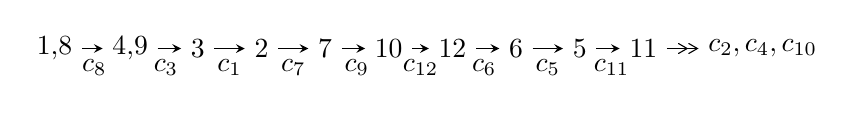
\begin{tikzpicture}[x=23pt, y=7pt]
	% node
	\node (A0) at (-1/8, 0) {1,8};
	\node (A1) at (17/16, 0) {4,9};
	\node (A2) at (17/8, 0) {3};
	\node (A3) at (25/8, 0) {2};
	\node (A4) at (33/8, 0) {7};
	\node (A5) at (41/8, 0) {10};
	\node (A6) at (49/8, 0) {12};
	\node (A7) at (57/8, 0) {6};
	\node (A8) at (65/8, 0) {5};
	\node (A9) at (73/8, 0) {11};
	\node (C1) at (1/2, -1) {$c_{8}$};
	\node (C2) at (13/8, -1) {$c_{3}$};
	\node (C3) at (21/8, -1) {$c_{1}$};
	\node (C4) at (29/8, -1) {$c_{7}$};
	\node (C5) at (37/8, -1) {$c_{9}$};
	\node (C6) at (45/8, -1) {$c_{12}$};
	\node (C7) at (53/8, -1) {$c_{6}$};
	\node (C8) at (61/8, -1) {$c_{5}$};
	\node (C9) at (69/8, -1) {$c_{11}$};
	\node (A10) at (11, 0) {$c_{2},c_{4},c_{10}$};

	% edge
	\draw[->,>=stealth]	
	(A0) edge (A1) (A1) edge (A2) (A2) edge (A3) (A3) edge (A4) (A4) edge (A5) (A5) edge (A6) (A6) edge (A7) (A7) edge (A8) (A8) edge (A9) ;
	\draw[->>,>={angle 60}]	
	(A9) edge (A10);
\end{tikzpicture} \\ 

\end{tabular} \\

\footnotetext{
The image of knot diagram is generated by the software ``\textbf{Draw programme}" developed by Andrew Bartholomew(\url{http://www.layer8.co.uk/maths/draw/index.htm\#Running-draw}), where we modified some parts for our purpose(\url{https://github.com/CATsTAILs/LinksPainter}).
}\phantom \\ \newline 
\centering \textbf{Ideals for irreducible components\footnotemark of $X_{\text{par}}$} 
 
\begin{align*}
I^u_{1}&=\langle 
2.14647\times10^{625} u^{136}-1.57204\times10^{626} u^{135}+\cdots+5.04273\times10^{627} b+2.01485\times10^{628},\\
\phantom{I^u_{1}}&\phantom{= \langle  }-9.52837\times10^{628} u^{136}+5.76897\times10^{629} u^{135}+\cdots+5.60247\times10^{630} a-2.60191\times10^{633},\\
\phantom{I^u_{1}}&\phantom{= \langle  }u^{137}-8 u^{136}+\cdots+109806 u+32219\rangle \\
I^u_{2}&=\langle 
969227805421 u^{29}+4997352190301 u^{28}+\cdots+7614592375217 b-1781800267381,\\
\phantom{I^u_{2}}&\phantom{= \langle  }-8214623303611 u^{29}-14241638447196 u^{28}+\cdots+7614592375217 a-12651568687672,\\
\phantom{I^u_{2}}&\phantom{= \langle  }u^{30}+u^{29}+\cdots+2 u+1\rangle \\
\\
\end{align*}
\raggedright * 2 irreducible components of $\dim_{\mathbb{C}}=0$, with total 167 representations.\\
\footnotetext{All coefficients of polynomials are rational numbers. But the coefficients are sometimes approximated in decimal forms when there is not enough margin.}
\newpage
\renewcommand{\arraystretch}{1}
\centering \section*{I. $I^u_{1}= \langle 2.15\times10^{625} u^{136}-1.57\times10^{626} u^{135}+\cdots+5.04\times10^{627} b+2.01\times10^{628},\;-9.53\times10^{628} u^{136}+5.77\times10^{629} u^{135}+\cdots+5.60\times10^{630} a-2.60\times10^{633},\;u^{137}-8 u^{136}+\cdots+109806 u+32219 \rangle$}
\flushleft \textbf{(i) Arc colorings}\\
\begin{tabular}{m{7pt} m{180pt} m{7pt} m{180pt} }
\flushright $a_{1}=$&$\begin{pmatrix}0\\u\end{pmatrix}$ \\
\flushright $a_{8}=$&$\begin{pmatrix}1\\0\end{pmatrix}$ \\
\flushright $a_{4}=$&$\begin{pmatrix}0.0170074 u^{136}-0.102972 u^{135}+\cdots+1977.46 u+464.422\\-0.00425657 u^{136}+0.0311744 u^{135}+\cdots-54.0695 u-3.99556\end{pmatrix}$ \\
\flushright $a_{9}=$&$\begin{pmatrix}1\\u^2\end{pmatrix}$ \\
\flushright $a_{3}=$&$\begin{pmatrix}0.0127509 u^{136}-0.0717974 u^{135}+\cdots+1923.39 u+460.426\\-0.00425657 u^{136}+0.0311744 u^{135}+\cdots-54.0695 u-3.99556\end{pmatrix}$ \\
\flushright $a_{2}=$&$\begin{pmatrix}0.104079 u^{136}-0.731582 u^{135}+\cdots+5658.43 u+962.800\\0.0141435 u^{136}-0.160591 u^{135}+\cdots-4271.95 u-1197.54\end{pmatrix}$ \\
\flushright $a_{7}=$&$\begin{pmatrix}0.0204806 u^{136}-0.164745 u^{135}+\cdots-957.487 u-341.646\\0.0166880 u^{136}-0.118460 u^{135}+\cdots+830.580 u+151.032\end{pmatrix}$ \\
\flushright $a_{10}=$&$\begin{pmatrix}0.154685 u^{136}-1.10541 u^{135}+\cdots+7925.61 u+1193.45\\-0.0228178 u^{136}+0.0717336 u^{135}+\cdots-8356.37 u-2109.51\end{pmatrix}$ \\
\flushright $a_{12}=$&$\begin{pmatrix}u\\u^3+u\end{pmatrix}$ \\
\flushright $a_{6}=$&$\begin{pmatrix}0.0414287 u^{136}-0.278536 u^{135}+\cdots+3054.14 u+617.717\\0.0316584 u^{136}-0.266647 u^{135}+\cdots-1739.62 u-622.793\end{pmatrix}$ \\
\flushright $a_{5}=$&$\begin{pmatrix}-0.164628 u^{136}+1.24456 u^{135}+\cdots-2428.11 u+289.540\\0.0406849 u^{136}-0.234576 u^{135}+\cdots+6901.62 u+1587.49\end{pmatrix}$ \\
\flushright $a_{11}=$&$\begin{pmatrix}-0.148430 u^{136}+0.926021 u^{135}+\cdots-18759.7 u-4096.98\\-0.00521443 u^{136}+0.202164 u^{135}+\cdots+12862.6 u+3478.39\end{pmatrix}$\\&\end{tabular}
\flushleft \textbf{(ii) Obstruction class $= -1$}\\~\\
\flushleft \textbf{(iii) Cusp Shapes $= 0.0777998 u^{136}-0.574500 u^{135}+\cdots+4442.71 u+535.291$}\\~\\
\newpage\renewcommand{\arraystretch}{1}
\flushleft \textbf{(iv) u-Polynomials at the component}\newline \\
\begin{tabular}{m{50pt}|m{274pt}}
Crossings & \hspace{64pt}u-Polynomials at each crossing \\
\hline $$\begin{aligned}c_{1}\end{aligned}$$&$\begin{aligned}
&u^{137}+51 u^{136}+\cdots+28 u+1
\end{aligned}$\\
\hline $$\begin{aligned}c_{2},c_{5}\end{aligned}$$&$\begin{aligned}
&u^{137}+3 u^{136}+\cdots-10 u+1
\end{aligned}$\\
\hline $$\begin{aligned}c_{3},c_{7}\end{aligned}$$&$\begin{aligned}
&u^{137}+u^{136}+\cdots-450658 u+20477
\end{aligned}$\\
\hline $$\begin{aligned}c_{4},c_{10}\end{aligned}$$&$\begin{aligned}
&u^{137}- u^{136}+\cdots+6 u^2+1
\end{aligned}$\\
\hline $$\begin{aligned}c_{6}\end{aligned}$$&$\begin{aligned}
&u^{137}-2 u^{136}+\cdots-4683 u+2473
\end{aligned}$\\
\hline $$\begin{aligned}c_{8},c_{12}\end{aligned}$$&$\begin{aligned}
&u^{137}-8 u^{136}+\cdots+109806 u+32219
\end{aligned}$\\
\hline $$\begin{aligned}c_{9}\end{aligned}$$&$\begin{aligned}
&u^{137}+16 u^{136}+\cdots+3863 u+251
\end{aligned}$\\
\hline $$\begin{aligned}c_{11}\end{aligned}$$&$\begin{aligned}
&u^{137}-63 u^{136}+\cdots-12 u+1
\end{aligned}$\\
\hline
\end{tabular}\\~\\
\newpage\renewcommand{\arraystretch}{1}
\flushleft \textbf{(v) Riley Polynomials at the component}\newline \\
\begin{tabular}{m{50pt}|m{274pt}}
Crossings & \hspace{64pt}Riley Polynomials at each crossing \\
\hline $$\begin{aligned}c_{1}\end{aligned}$$&$\begin{aligned}
&y^{137}+85 y^{136}+\cdots-8004 y-1
\end{aligned}$\\
\hline $$\begin{aligned}c_{2},c_{5}\end{aligned}$$&$\begin{aligned}
&y^{137}-51 y^{136}+\cdots+28 y-1
\end{aligned}$\\
\hline $$\begin{aligned}c_{3},c_{7}\end{aligned}$$&$\begin{aligned}
&y^{137}+115 y^{136}+\cdots-17103469262 y-419307529
\end{aligned}$\\
\hline $$\begin{aligned}c_{4},c_{10}\end{aligned}$$&$\begin{aligned}
&y^{137}+63 y^{136}+\cdots-12 y-1
\end{aligned}$\\
\hline $$\begin{aligned}c_{6}\end{aligned}$$&$\begin{aligned}
&y^{137}-12 y^{136}+\cdots+196459991 y-6115729
\end{aligned}$\\
\hline $$\begin{aligned}c_{8},c_{12}\end{aligned}$$&$\begin{aligned}
&y^{137}+118 y^{136}+\cdots+87908229568 y-1038063961
\end{aligned}$\\
\hline $$\begin{aligned}c_{9}\end{aligned}$$&$\begin{aligned}
&y^{137}-22 y^{136}+\cdots+8590039 y-63001
\end{aligned}$\\
\hline $$\begin{aligned}c_{11}\end{aligned}$$&$\begin{aligned}
&y^{137}+39 y^{136}+\cdots+44 y-1
\end{aligned}$\\
\hline
\end{tabular}\\~\\
\newpage\flushleft \textbf{(vi) Complex Volumes and Cusp Shapes}
$$\begin{array}{c|c|c}  
\text{Solutions to }I^u_{1}& \I (\text{vol} + \sqrt{-1}CS) & \text{Cusp shape}\\
 \hline 
\begin{aligned}
u &= -0.600215 + 0.825884 I \\
a &= \phantom{-}0.341214 + 0.182187 I \\
b &= \phantom{-}0.0429581 + 0.0446813 I\end{aligned}
 & -0.76985 + 2.36523 I & \phantom{-0.000000 } 0 \\ \hline\begin{aligned}
u &= -0.600215 - 0.825884 I \\
a &= \phantom{-}0.341214 - 0.182187 I \\
b &= \phantom{-}0.0429581 - 0.0446813 I\end{aligned}
 & -0.76985 - 2.36523 I & \phantom{-0.000000 } 0 \\ \hline\begin{aligned}
u &= \phantom{-}0.276628 + 0.934882 I \\
a &= \phantom{-}0.134951 + 0.863792 I \\
b &= -0.754988 - 0.080370 I\end{aligned}
 & \phantom{-}0.027372 - 1.013400 I & \phantom{-0.000000 } 0 \\ \hline\begin{aligned}
u &= \phantom{-}0.276628 - 0.934882 I \\
a &= \phantom{-}0.134951 - 0.863792 I \\
b &= -0.754988 + 0.080370 I\end{aligned}
 & \phantom{-}0.027372 + 1.013400 I & \phantom{-0.000000 } 0 \\ \hline\begin{aligned}
u &= \phantom{-}0.277443 + 1.042560 I \\
a &= -0.56568 + 1.72089 I \\
b &= \phantom{-}0.509378 - 0.961639 I\end{aligned}
 & \phantom{-}2.76698 + 4.14223 I & \phantom{-0.000000 } 0 \\ \hline\begin{aligned}
u &= \phantom{-}0.277443 - 1.042560 I \\
a &= -0.56568 - 1.72089 I \\
b &= \phantom{-}0.509378 + 0.961639 I\end{aligned}
 & \phantom{-}2.76698 - 4.14223 I & \phantom{-0.000000 } 0 \\ \hline\begin{aligned}
u &= -0.810726 + 0.376962 I \\
a &= \phantom{-}0.625383 + 0.386915 I \\
b &= \phantom{-}0.719560 - 0.588147 I\end{aligned}
 & -4.43117 + 3.80080 I & \phantom{-0.000000 } 0 \\ \hline\begin{aligned}
u &= -0.810726 - 0.376962 I \\
a &= \phantom{-}0.625383 - 0.386915 I \\
b &= \phantom{-}0.719560 + 0.588147 I\end{aligned}
 & -4.43117 - 3.80080 I & \phantom{-0.000000 } 0 \\ \hline\begin{aligned}
u &= \phantom{-}0.405570 + 0.762614 I \\
a &= -0.577183 - 0.645655 I \\
b &= \phantom{-}0.565672 + 0.632820 I\end{aligned}
 & \phantom{-}2.17077 - 6.60754 I & \phantom{-0.000000 } 0 \\ \hline\begin{aligned}
u &= \phantom{-}0.405570 - 0.762614 I \\
a &= -0.577183 + 0.645655 I \\
b &= \phantom{-}0.565672 - 0.632820 I\end{aligned}
 & \phantom{-}2.17077 + 6.60754 I & \phantom{-0.000000 } 0\\
 \hline 
 \end{array}$$\newpage$$\begin{array}{c|c|c}  
\text{Solutions to }I^u_{1}& \I (\text{vol} + \sqrt{-1}CS) & \text{Cusp shape}\\
 \hline 
\begin{aligned}
u &= -0.480617 + 0.678664 I \\
a &= \phantom{-}0.319527 - 0.525767 I \\
b &= -0.342427 + 0.558103 I\end{aligned}
 & -0.09125 + 2.10745 I & \phantom{-0.000000 } 0 \\ \hline\begin{aligned}
u &= -0.480617 - 0.678664 I \\
a &= \phantom{-}0.319527 + 0.525767 I \\
b &= -0.342427 - 0.558103 I\end{aligned}
 & -0.09125 - 2.10745 I & \phantom{-0.000000 } 0 \\ \hline\begin{aligned}
u &= \phantom{-}0.365595 + 1.115550 I \\
a &= -0.320099 - 0.727207 I \\
b &= -0.124434 + 0.427629 I\end{aligned}
 & \phantom{-}3.82283 + 0.95919 I & \phantom{-0.000000 } 0 \\ \hline\begin{aligned}
u &= \phantom{-}0.365595 - 1.115550 I \\
a &= -0.320099 + 0.727207 I \\
b &= -0.124434 - 0.427629 I\end{aligned}
 & \phantom{-}3.82283 - 0.95919 I & \phantom{-0.000000 } 0 \\ \hline\begin{aligned}
u &= \phantom{-}1.104240 + 0.401110 I \\
a &= \phantom{-}0.113677 - 0.484296 I \\
b &= \phantom{-}0.282562 + 1.184250 I\end{aligned}
 & \phantom{-}3.38915 - 7.43186 I & \phantom{-0.000000 } 0 \\ \hline\begin{aligned}
u &= \phantom{-}1.104240 - 0.401110 I \\
a &= \phantom{-}0.113677 + 0.484296 I \\
b &= \phantom{-}0.282562 - 1.184250 I\end{aligned}
 & \phantom{-}3.38915 + 7.43186 I & \phantom{-0.000000 } 0 \\ \hline\begin{aligned}
u &= \phantom{-}0.250630 + 1.162460 I \\
a &= -0.58140 + 2.21392 I \\
b &= \phantom{-}0.022548 - 1.349140 I\end{aligned}
 & \phantom{-}5.36671 - 3.68922 I & \phantom{-0.000000 } 0 \\ \hline\begin{aligned}
u &= \phantom{-}0.250630 - 1.162460 I \\
a &= -0.58140 - 2.21392 I \\
b &= \phantom{-}0.022548 + 1.349140 I\end{aligned}
 & \phantom{-}5.36671 + 3.68922 I & \phantom{-0.000000 } 0 \\ \hline\begin{aligned}
u &= \phantom{-}0.509415 + 1.076190 I \\
a &= \phantom{-}0.524591 + 0.518478 I \\
b &= -0.886419 + 0.425051 I\end{aligned}
 & -1.57184 - 5.75032 I & \phantom{-0.000000 } 0 \\ \hline\begin{aligned}
u &= \phantom{-}0.509415 - 1.076190 I \\
a &= \phantom{-}0.524591 - 0.518478 I \\
b &= -0.886419 - 0.425051 I\end{aligned}
 & -1.57184 + 5.75032 I & \phantom{-0.000000 } 0\\
 \hline 
 \end{array}$$\newpage$$\begin{array}{c|c|c}  
\text{Solutions to }I^u_{1}& \I (\text{vol} + \sqrt{-1}CS) & \text{Cusp shape}\\
 \hline 
\begin{aligned}
u &= -0.584119 + 1.041150 I \\
a &= -0.460558 + 0.276017 I \\
b &= \phantom{-}0.676065 + 0.560471 I\end{aligned}
 & -2.46994 + 1.25079 I & \phantom{-0.000000 } 0 \\ \hline\begin{aligned}
u &= -0.584119 - 1.041150 I \\
a &= -0.460558 - 0.276017 I \\
b &= \phantom{-}0.676065 - 0.560471 I\end{aligned}
 & -2.46994 - 1.25079 I & \phantom{-0.000000 } 0 \\ \hline\begin{aligned}
u &= -0.144415 + 1.190800 I \\
a &= \phantom{-}0.457281 - 0.122460 I \\
b &= -1.212230 + 0.285741 I\end{aligned}
 & \phantom{-}1.47034 + 1.58354 I & \phantom{-0.000000 } 0 \\ \hline\begin{aligned}
u &= -0.144415 - 1.190800 I \\
a &= \phantom{-}0.457281 + 0.122460 I \\
b &= -1.212230 - 0.285741 I\end{aligned}
 & \phantom{-}1.47034 - 1.58354 I & \phantom{-0.000000 } 0 \\ \hline\begin{aligned}
u &= -0.753738 + 0.257933 I \\
a &= \phantom{-}0.795857 - 0.701646 I \\
b &= \phantom{-}0.576601 + 0.874596 I\end{aligned}
 & -3.62189 - 1.01410 I & \phantom{-0.000000 } 0 \\ \hline\begin{aligned}
u &= -0.753738 - 0.257933 I \\
a &= \phantom{-}0.795857 + 0.701646 I \\
b &= \phantom{-}0.576601 - 0.874596 I\end{aligned}
 & -3.62189 + 1.01410 I & \phantom{-0.000000 } 0 \\ \hline\begin{aligned}
u &= -0.335437 + 1.157330 I \\
a &= \phantom{-}0.25846 + 1.95888 I \\
b &= -0.141406 - 0.950478 I\end{aligned}
 & \phantom{-}0.252574 + 1.080440 I & \phantom{-0.000000 } 0 \\ \hline\begin{aligned}
u &= -0.335437 - 1.157330 I \\
a &= \phantom{-}0.25846 - 1.95888 I \\
b &= -0.141406 + 0.950478 I\end{aligned}
 & \phantom{-}0.252574 - 1.080440 I & \phantom{-0.000000 } 0 \\ \hline\begin{aligned}
u &= \phantom{-}0.173074 + 1.196750 I \\
a &= -0.613118 - 0.319995 I \\
b &= \phantom{-}1.36621 + 0.38306 I\end{aligned}
 & \phantom{-}3.36982 - 6.59254 I & \phantom{-0.000000 } 0 \\ \hline\begin{aligned}
u &= \phantom{-}0.173074 - 1.196750 I \\
a &= -0.613118 + 0.319995 I \\
b &= \phantom{-}1.36621 - 0.38306 I\end{aligned}
 & \phantom{-}3.36982 + 6.59254 I & \phantom{-0.000000 } 0\\
 \hline 
 \end{array}$$\newpage$$\begin{array}{c|c|c}  
\text{Solutions to }I^u_{1}& \I (\text{vol} + \sqrt{-1}CS) & \text{Cusp shape}\\
 \hline 
\begin{aligned}
u &= \phantom{-}0.252583 + 1.193810 I \\
a &= -0.48841 + 2.77901 I \\
b &= -0.325330 - 1.160690 I\end{aligned}
 & \phantom{-}0.75973 - 9.92657 I & \phantom{-0.000000 } 0 \\ \hline\begin{aligned}
u &= \phantom{-}0.252583 - 1.193810 I \\
a &= -0.48841 - 2.77901 I \\
b &= -0.325330 + 1.160690 I\end{aligned}
 & \phantom{-}0.75973 + 9.92657 I & \phantom{-0.000000 } 0 \\ \hline\begin{aligned}
u &= \phantom{-}0.401665 + 0.667335 I \\
a &= -0.191681 - 0.810457 I \\
b &= \phantom{-}0.128406 + 0.873969 I\end{aligned}
 & \phantom{-}3.65193 + 0.66673 I & \phantom{-0.000000 } 0 \\ \hline\begin{aligned}
u &= \phantom{-}0.401665 - 0.667335 I \\
a &= -0.191681 + 0.810457 I \\
b &= \phantom{-}0.128406 - 0.873969 I\end{aligned}
 & \phantom{-}3.65193 - 0.66673 I & \phantom{-0.000000 } 0 \\ \hline\begin{aligned}
u &= -0.259460 + 1.196040 I \\
a &= \phantom{-}0.33681 + 2.61041 I \\
b &= \phantom{-}0.245278 - 1.105050 I\end{aligned}
 & -0.75094 + 4.51996 I & \phantom{-0.000000 } 0 \\ \hline\begin{aligned}
u &= -0.259460 - 1.196040 I \\
a &= \phantom{-}0.33681 - 2.61041 I \\
b &= \phantom{-}0.245278 + 1.105050 I\end{aligned}
 & -0.75094 - 4.51996 I & \phantom{-0.000000 } 0 \\ \hline\begin{aligned}
u &= -0.043599 + 1.224900 I \\
a &= -0.081497 + 0.491243 I \\
b &= -0.773182 + 0.003155 I\end{aligned}
 & \phantom{-}0.851004 - 0.795140 I & \phantom{-0.000000 } 0 \\ \hline\begin{aligned}
u &= -0.043599 - 1.224900 I \\
a &= -0.081497 - 0.491243 I \\
b &= -0.773182 - 0.003155 I\end{aligned}
 & \phantom{-}0.851004 + 0.795140 I & \phantom{-0.000000 } 0 \\ \hline\begin{aligned}
u &= -0.272248 + 1.198580 I \\
a &= \phantom{-}1.73020 + 1.65034 I \\
b &= \phantom{-}0.246093 - 1.307720 I\end{aligned}
 & \phantom{-}6.31626 + 8.78487 I & \phantom{-0.000000 } 0 \\ \hline\begin{aligned}
u &= -0.272248 - 1.198580 I \\
a &= \phantom{-}1.73020 - 1.65034 I \\
b &= \phantom{-}0.246093 + 1.307720 I\end{aligned}
 & \phantom{-}6.31626 - 8.78487 I & \phantom{-0.000000 } 0\\
 \hline 
 \end{array}$$\newpage$$\begin{array}{c|c|c}  
\text{Solutions to }I^u_{1}& \I (\text{vol} + \sqrt{-1}CS) & \text{Cusp shape}\\
 \hline 
\begin{aligned}
u &= \phantom{-}0.258801 + 1.202340 I \\
a &= -1.24707 + 1.88429 I \\
b &= -0.356991 - 1.338480 I\end{aligned}
 & \phantom{-}5.05012 - 5.03282 I & \phantom{-0.000000 } 0 \\ \hline\begin{aligned}
u &= \phantom{-}0.258801 - 1.202340 I \\
a &= -1.24707 - 1.88429 I \\
b &= -0.356991 + 1.338480 I\end{aligned}
 & \phantom{-}5.05012 + 5.03282 I & \phantom{-0.000000 } 0 \\ \hline\begin{aligned}
u &= \phantom{-}0.721061 + 0.261174 I \\
a &= -0.765255 + 0.337826 I \\
b &= -0.857391 - 0.405574 I\end{aligned}
 & -3.95395 + 1.20522 I & \phantom{-0.000000 } 0 \\ \hline\begin{aligned}
u &= \phantom{-}0.721061 - 0.261174 I \\
a &= -0.765255 - 0.337826 I \\
b &= -0.857391 + 0.405574 I\end{aligned}
 & -3.95395 - 1.20522 I & \phantom{-0.000000 } 0 \\ \hline\begin{aligned}
u &= -0.212759 + 1.219960 I \\
a &= \phantom{-}0.39889 + 2.02793 I \\
b &= \phantom{-}0.61084 - 1.77061 I\end{aligned}
 & \phantom{-}7.76381 + 1.99463 I & \phantom{-0.000000 } 0 \\ \hline\begin{aligned}
u &= -0.212759 - 1.219960 I \\
a &= \phantom{-}0.39889 - 2.02793 I \\
b &= \phantom{-}0.61084 + 1.77061 I\end{aligned}
 & \phantom{-}7.76381 - 1.99463 I & \phantom{-0.000000 } 0 \\ \hline\begin{aligned}
u &= -0.286333 + 1.210290 I \\
a &= \phantom{-}1.61945 + 0.94113 I \\
b &= \phantom{-}0.169209 - 1.077120 I\end{aligned}
 & \phantom{-}6.76255 + 2.94842 I & \phantom{-0.000000 } 0 \\ \hline\begin{aligned}
u &= -0.286333 - 1.210290 I \\
a &= \phantom{-}1.61945 - 0.94113 I \\
b &= \phantom{-}0.169209 + 1.077120 I\end{aligned}
 & \phantom{-}6.76255 - 2.94842 I & \phantom{-0.000000 } 0 \\ \hline\begin{aligned}
u &= \phantom{-}0.243282 + 1.224860 I \\
a &= -0.64177 + 1.67068 I \\
b &= -0.60807 - 1.39180 I\end{aligned}
 & \phantom{-}5.39433 - 5.32907 I & \phantom{-0.000000 } 0 \\ \hline\begin{aligned}
u &= \phantom{-}0.243282 - 1.224860 I \\
a &= -0.64177 - 1.67068 I \\
b &= -0.60807 + 1.39180 I\end{aligned}
 & \phantom{-}5.39433 + 5.32907 I & \phantom{-0.000000 } 0\\
 \hline 
 \end{array}$$\newpage$$\begin{array}{c|c|c}  
\text{Solutions to }I^u_{1}& \I (\text{vol} + \sqrt{-1}CS) & \text{Cusp shape}\\
 \hline 
\begin{aligned}
u &= \phantom{-}0.699243 + 0.265046 I \\
a &= -0.902246 - 0.458831 I \\
b &= -0.627171 + 1.038880 I\end{aligned}
 & -2.08258 + 6.56291 I & \phantom{-0.000000 } 0 \\ \hline\begin{aligned}
u &= \phantom{-}0.699243 - 0.265046 I \\
a &= -0.902246 + 0.458831 I \\
b &= -0.627171 - 1.038880 I\end{aligned}
 & -2.08258 - 6.56291 I & \phantom{-0.000000 } 0 \\ \hline\begin{aligned}
u &= \phantom{-}0.133455 + 1.251360 I \\
a &= \phantom{-}0.084175 - 0.523657 I \\
b &= \phantom{-}0.895480 + 0.648314 I\end{aligned}
 & \phantom{-}6.23673 + 0.17961 I & \phantom{-0.000000 } 0 \\ \hline\begin{aligned}
u &= \phantom{-}0.133455 - 1.251360 I \\
a &= \phantom{-}0.084175 + 0.523657 I \\
b &= \phantom{-}0.895480 - 0.648314 I\end{aligned}
 & \phantom{-}6.23673 - 0.17961 I & \phantom{-0.000000 } 0 \\ \hline\begin{aligned}
u &= -0.221879 + 1.250790 I \\
a &= \phantom{-}0.11965 + 1.70945 I \\
b &= \phantom{-}1.01410 - 1.57896 I\end{aligned}
 & \phantom{-}7.61960 + 8.66163 I & \phantom{-0.000000 } 0 \\ \hline\begin{aligned}
u &= -0.221879 - 1.250790 I \\
a &= \phantom{-}0.11965 - 1.70945 I \\
b &= \phantom{-}1.01410 + 1.57896 I\end{aligned}
 & \phantom{-}7.61960 - 8.66163 I & \phantom{-0.000000 } 0 \\ \hline\begin{aligned}
u &= \phantom{-}0.301681 + 1.242530 I \\
a &= -0.725555 + 0.385722 I \\
b &= -0.484597 - 0.574971 I\end{aligned}
 & \phantom{-}5.79279 - 5.78435 I & \phantom{-0.000000 } 0 \\ \hline\begin{aligned}
u &= \phantom{-}0.301681 - 1.242530 I \\
a &= -0.725555 - 0.385722 I \\
b &= -0.484597 + 0.574971 I\end{aligned}
 & \phantom{-}5.79279 + 5.78435 I & \phantom{-0.000000 } 0 \\ \hline\begin{aligned}
u &= -0.063134 + 1.281760 I \\
a &= -1.23684 - 2.14792 I \\
b &= -0.011264 + 1.216080 I\end{aligned}
 & \phantom{-}8.36571 - 4.84327 I & \phantom{-0.000000 } 0 \\ \hline\begin{aligned}
u &= -0.063134 - 1.281760 I \\
a &= -1.23684 + 2.14792 I \\
b &= -0.011264 - 1.216080 I\end{aligned}
 & \phantom{-}8.36571 + 4.84327 I & \phantom{-0.000000 } 0\\
 \hline 
 \end{array}$$\newpage$$\begin{array}{c|c|c}  
\text{Solutions to }I^u_{1}& \I (\text{vol} + \sqrt{-1}CS) & \text{Cusp shape}\\
 \hline 
\begin{aligned}
u &= -1.134330 + 0.617531 I \\
a &= -0.127196 - 0.486382 I \\
b &= -0.126525 + 1.070720 I\end{aligned}
 & \phantom{-}0.54578 + 1.90911 I & \phantom{-0.000000 } 0 \\ \hline\begin{aligned}
u &= -1.134330 - 0.617531 I \\
a &= -0.127196 + 0.486382 I \\
b &= -0.126525 - 1.070720 I\end{aligned}
 & \phantom{-}0.54578 - 1.90911 I & \phantom{-0.000000 } 0 \\ \hline\begin{aligned}
u &= \phantom{-}0.275113 + 1.263970 I \\
a &= -0.281993 + 0.830321 I \\
b &= -0.913446 - 0.799643 I\end{aligned}
 & \phantom{-}5.75402 - 5.70433 I & \phantom{-0.000000 } 0 \\ \hline\begin{aligned}
u &= \phantom{-}0.275113 - 1.263970 I \\
a &= -0.281993 - 0.830321 I \\
b &= -0.913446 + 0.799643 I\end{aligned}
 & \phantom{-}5.75402 + 5.70433 I & \phantom{-0.000000 } 0 \\ \hline\begin{aligned}
u &= \phantom{-}0.069435 + 1.294050 I \\
a &= \phantom{-}0.579558 + 0.665158 I \\
b &= \phantom{-}0.445851 - 0.025283 I\end{aligned}
 & \phantom{-}2.09940 + 6.03519 I & \phantom{-0.000000 } 0 \\ \hline\begin{aligned}
u &= \phantom{-}0.069435 - 1.294050 I \\
a &= \phantom{-}0.579558 - 0.665158 I \\
b &= \phantom{-}0.445851 + 0.025283 I\end{aligned}
 & \phantom{-}2.09940 - 6.03519 I & \phantom{-0.000000 } 0 \\ \hline\begin{aligned}
u &= -0.026064 + 1.295990 I \\
a &= -0.48548 - 2.61453 I \\
b &= -0.008508 + 1.375680 I\end{aligned}
 & \phantom{-}9.41866 + 1.21222 I & \phantom{-0.000000 } 0 \\ \hline\begin{aligned}
u &= -0.026064 - 1.295990 I \\
a &= -0.48548 + 2.61453 I \\
b &= -0.008508 - 1.375680 I\end{aligned}
 & \phantom{-}9.41866 - 1.21222 I & \phantom{-0.000000 } 0 \\ \hline\begin{aligned}
u &= \phantom{-}0.081715 + 1.302440 I \\
a &= \phantom{-}0.81523 - 1.72233 I \\
b &= \phantom{-}0.201606 + 1.228170 I\end{aligned}
 & \phantom{-}6.74367 + 0.78269 I & \phantom{-0.000000 } 0 \\ \hline\begin{aligned}
u &= \phantom{-}0.081715 - 1.302440 I \\
a &= \phantom{-}0.81523 + 1.72233 I \\
b &= \phantom{-}0.201606 - 1.228170 I\end{aligned}
 & \phantom{-}6.74367 - 0.78269 I & \phantom{-0.000000 } 0\\
 \hline 
 \end{array}$$\newpage$$\begin{array}{c|c|c}  
\text{Solutions to }I^u_{1}& \I (\text{vol} + \sqrt{-1}CS) & \text{Cusp shape}\\
 \hline 
\begin{aligned}
u &= \phantom{-}1.297150 + 0.204185 I \\
a &= -0.219346 + 0.377698 I \\
b &= -0.388633 - 1.344330 I\end{aligned}
 & \phantom{-}2.21246 - 12.85340 I & \phantom{-0.000000 } 0 \\ \hline\begin{aligned}
u &= \phantom{-}1.297150 - 0.204185 I \\
a &= -0.219346 - 0.377698 I \\
b &= -0.388633 + 1.344330 I\end{aligned}
 & \phantom{-}2.21246 + 12.85340 I & \phantom{-0.000000 } 0 \\ \hline\begin{aligned}
u &= -0.677201 + 0.041589 I \\
a &= \phantom{-}0.80512 - 1.49239 I \\
b &= \phantom{-}0.677223 + 0.180341 I\end{aligned}
 & -3.72494 + 3.01705 I & -13.21532 - 1.96138 I \\ \hline\begin{aligned}
u &= -0.677201 - 0.041589 I \\
a &= \phantom{-}0.80512 + 1.49239 I \\
b &= \phantom{-}0.677223 - 0.180341 I\end{aligned}
 & -3.72494 - 3.01705 I & -13.21532 + 1.96138 I \\ \hline\begin{aligned}
u &= \phantom{-}0.117160 + 1.322660 I \\
a &= \phantom{-}0.37918 - 1.50554 I \\
b &= \phantom{-}0.49170 + 1.36391 I\end{aligned}
 & \phantom{-}6.72024 + 0.53681 I & \phantom{-0.000000 } 0 \\ \hline\begin{aligned}
u &= \phantom{-}0.117160 - 1.322660 I \\
a &= \phantom{-}0.37918 + 1.50554 I \\
b &= \phantom{-}0.49170 - 1.36391 I\end{aligned}
 & \phantom{-}6.72024 - 0.53681 I & \phantom{-0.000000 } 0 \\ \hline\begin{aligned}
u &= -0.161042 + 1.342350 I \\
a &= -0.05597 - 1.61600 I \\
b &= -0.80150 + 1.70452 I\end{aligned}
 & \phantom{-}8.26014 + 3.01778 I & \phantom{-0.000000 } 0 \\ \hline\begin{aligned}
u &= -0.161042 - 1.342350 I \\
a &= -0.05597 + 1.61600 I \\
b &= -0.80150 - 1.70452 I\end{aligned}
 & \phantom{-}8.26014 - 3.01778 I & \phantom{-0.000000 } 0 \\ \hline\begin{aligned}
u &= -0.407256 + 1.294530 I \\
a &= \phantom{-}0.026183 - 0.389081 I \\
b &= \phantom{-}0.680029 + 0.369673 I\end{aligned}
 & \phantom{-}1.35104 + 3.81155 I & \phantom{-0.000000 } 0 \\ \hline\begin{aligned}
u &= -0.407256 - 1.294530 I \\
a &= \phantom{-}0.026183 + 0.389081 I \\
b &= \phantom{-}0.680029 - 0.369673 I\end{aligned}
 & \phantom{-}1.35104 - 3.81155 I & \phantom{-0.000000 } 0\\
 \hline 
 \end{array}$$\newpage$$\begin{array}{c|c|c}  
\text{Solutions to }I^u_{1}& \I (\text{vol} + \sqrt{-1}CS) & \text{Cusp shape}\\
 \hline 
\begin{aligned}
u &= -0.610534 + 0.186046 I \\
a &= \phantom{-}0.445388 + 0.957310 I \\
b &= -0.03359 + 1.41643 I\end{aligned}
 & \phantom{-}3.24778 - 5.49829 I & -5.00006 + 6.13472 I \\ \hline\begin{aligned}
u &= -0.610534 - 0.186046 I \\
a &= \phantom{-}0.445388 - 0.957310 I \\
b &= -0.03359 - 1.41643 I\end{aligned}
 & \phantom{-}3.24778 + 5.49829 I & -5.00006 - 6.13472 I \\ \hline\begin{aligned}
u &= \phantom{-}0.286945 + 1.332370 I \\
a &= \phantom{-}0.527188 + 0.317971 I \\
b &= -1.57004 - 0.11173 I\end{aligned}
 & \phantom{-}2.31371 - 11.85850 I & \phantom{-0.000000 } 0 \\ \hline\begin{aligned}
u &= \phantom{-}0.286945 - 1.332370 I \\
a &= \phantom{-}0.527188 - 0.317971 I \\
b &= -1.57004 + 0.11173 I\end{aligned}
 & \phantom{-}2.31371 + 11.85850 I & \phantom{-0.000000 } 0 \\ \hline\begin{aligned}
u &= -0.306302 + 1.331350 I \\
a &= -0.395801 + 0.146440 I \\
b &= \phantom{-}1.368200 + 0.027238 I\end{aligned}
 & \phantom{-}0.67456 + 6.63501 I & \phantom{-0.000000 } 0 \\ \hline\begin{aligned}
u &= -0.306302 - 1.331350 I \\
a &= -0.395801 - 0.146440 I \\
b &= \phantom{-}1.368200 - 0.027238 I\end{aligned}
 & \phantom{-}0.67456 - 6.63501 I & \phantom{-0.000000 } 0 \\ \hline\begin{aligned}
u &= \phantom{-}0.626514 + 0.050151 I \\
a &= -0.84200 - 1.70554 I \\
b &= -0.811167 + 0.011205 I\end{aligned}
 & -2.10741 - 8.46095 I & -10.29053 + 6.92192 I \\ \hline\begin{aligned}
u &= \phantom{-}0.626514 - 0.050151 I \\
a &= -0.84200 + 1.70554 I \\
b &= -0.811167 - 0.011205 I\end{aligned}
 & -2.10741 + 8.46095 I & -10.29053 - 6.92192 I \\ \hline\begin{aligned}
u &= \phantom{-}0.583255 + 0.219848 I \\
a &= -0.316978 + 0.624569 I \\
b &= -0.166804 + 1.320420 I\end{aligned}
 & \phantom{-}2.04697 + 1.89378 I & -8.30712 + 0. I\phantom{ +0.000000I} \\ \hline\begin{aligned}
u &= \phantom{-}0.583255 - 0.219848 I \\
a &= -0.316978 - 0.624569 I \\
b &= -0.166804 - 1.320420 I\end{aligned}
 & \phantom{-}2.04697 - 1.89378 I & -8.30712 + 0. I\phantom{ +0.000000I}\\
 \hline 
 \end{array}$$\newpage$$\begin{array}{c|c|c}  
\text{Solutions to }I^u_{1}& \I (\text{vol} + \sqrt{-1}CS) & \text{Cusp shape}\\
 \hline 
\begin{aligned}
u &= -0.606620 + 0.139527 I \\
a &= \phantom{-}0.267987 + 1.177840 I \\
b &= -0.266261 + 1.165630 I\end{aligned}
 & \phantom{-}3.51581 + 0.39606 I & -4.02934 - 2.78608 I \\ \hline\begin{aligned}
u &= -0.606620 - 0.139527 I \\
a &= \phantom{-}0.267987 - 1.177840 I \\
b &= -0.266261 - 1.165630 I\end{aligned}
 & \phantom{-}3.51581 - 0.39606 I & -4.02934 + 2.78608 I \\ \hline\begin{aligned}
u &= -0.157220 + 1.386930 I \\
a &= -0.20262 - 1.78566 I \\
b &= -0.43911 + 2.00856 I\end{aligned}
 & \phantom{-}8.39206 - 2.84568 I & \phantom{-0.000000 } 0 \\ \hline\begin{aligned}
u &= -0.157220 - 1.386930 I \\
a &= -0.20262 + 1.78566 I \\
b &= -0.43911 - 2.00856 I\end{aligned}
 & \phantom{-}8.39206 + 2.84568 I & \phantom{-0.000000 } 0 \\ \hline\begin{aligned}
u &= -1.365400 + 0.316476 I \\
a &= \phantom{-}0.260102 + 0.452500 I \\
b &= \phantom{-}0.343139 - 1.221160 I\end{aligned}
 & -0.43097 + 6.85078 I & \phantom{-0.000000 } 0 \\ \hline\begin{aligned}
u &= -1.365400 - 0.316476 I \\
a &= \phantom{-}0.260102 - 0.452500 I \\
b &= \phantom{-}0.343139 + 1.221160 I\end{aligned}
 & -0.43097 - 6.85078 I & \phantom{-0.000000 } 0 \\ \hline\begin{aligned}
u &= \phantom{-}0.583549 + 0.102512 I \\
a &= -0.136693 - 0.917007 I \\
b &= \phantom{-}0.696924 + 0.132143 I\end{aligned}
 & \phantom{-}0.25747 + 3.83112 I & -5.71601 - 2.49405 I \\ \hline\begin{aligned}
u &= \phantom{-}0.583549 - 0.102512 I \\
a &= -0.136693 + 0.917007 I \\
b &= \phantom{-}0.696924 - 0.132143 I\end{aligned}
 & \phantom{-}0.25747 - 3.83112 I & -5.71601 + 2.49405 I \\ \hline\begin{aligned}
u &= -0.531137 + 0.228329 I \\
a &= \phantom{-}0.154180 - 0.733272 I \\
b &= -0.525007 + 0.334915 I\end{aligned}
 & -1.23027 + 0.80713 I & -8.01143 - 3.82200 I \\ \hline\begin{aligned}
u &= -0.531137 - 0.228329 I \\
a &= \phantom{-}0.154180 + 0.733272 I \\
b &= -0.525007 - 0.334915 I\end{aligned}
 & -1.23027 - 0.80713 I & -8.01143 + 3.82200 I\\
 \hline 
 \end{array}$$\newpage$$\begin{array}{c|c|c}  
\text{Solutions to }I^u_{1}& \I (\text{vol} + \sqrt{-1}CS) & \text{Cusp shape}\\
 \hline 
\begin{aligned}
u &= \phantom{-}0.13412 + 1.42109 I \\
a &= \phantom{-}0.27480 - 1.72876 I \\
b &= \phantom{-}0.12100 + 1.91232 I\end{aligned}
 & \phantom{-}7.51590 - 0.56584 I & \phantom{-0.000000 } 0 \\ \hline\begin{aligned}
u &= \phantom{-}0.13412 - 1.42109 I \\
a &= \phantom{-}0.27480 + 1.72876 I \\
b &= \phantom{-}0.12100 - 1.91232 I\end{aligned}
 & \phantom{-}7.51590 + 0.56584 I & \phantom{-0.000000 } 0 \\ \hline\begin{aligned}
u &= \phantom{-}0.562181 + 0.080157 I \\
a &= -0.292233 + 1.307150 I \\
b &= \phantom{-}0.176536 + 0.354661 I\end{aligned}
 & \phantom{-}2.25523 + 2.39599 I & -5.21005 - 3.82646 I \\ \hline\begin{aligned}
u &= \phantom{-}0.562181 - 0.080157 I \\
a &= -0.292233 - 1.307150 I \\
b &= \phantom{-}0.176536 - 0.354661 I\end{aligned}
 & \phantom{-}2.25523 - 2.39599 I & -5.21005 + 3.82646 I \\ \hline\begin{aligned}
u &= \phantom{-}0.528989 + 0.104664 I \\
a &= \phantom{-}0.091902 + 1.360790 I \\
b &= -0.204011 + 0.867265 I\end{aligned}
 & \phantom{-}2.14967 + 2.60628 I & -6.80056 - 4.70746 I \\ \hline\begin{aligned}
u &= \phantom{-}0.528989 - 0.104664 I \\
a &= \phantom{-}0.091902 - 1.360790 I \\
b &= -0.204011 - 0.867265 I\end{aligned}
 & \phantom{-}2.14967 - 2.60628 I & -6.80056 + 4.70746 I \\ \hline\begin{aligned}
u &= \phantom{-}0.488642 + 0.156091 I \\
a &= \phantom{-}0.419703 + 1.008160 I \\
b &= -0.258118 + 1.102630 I\end{aligned}
 & \phantom{-}2.13489 + 2.49230 I & -4.55425 - 3.52768 I \\ \hline\begin{aligned}
u &= \phantom{-}0.488642 - 0.156091 I \\
a &= \phantom{-}0.419703 - 1.008160 I \\
b &= -0.258118 - 1.102630 I\end{aligned}
 & \phantom{-}2.13489 - 2.49230 I & -4.55425 + 3.52768 I \\ \hline\begin{aligned}
u &= \phantom{-}0.41429 + 1.47620 I \\
a &= \phantom{-}0.42248 - 1.73952 I \\
b &= \phantom{-}0.47672 + 1.49807 I\end{aligned}
 & \phantom{-}9.2931 - 12.6983 I & \phantom{-0.000000 } 0 \\ \hline\begin{aligned}
u &= \phantom{-}0.41429 - 1.47620 I \\
a &= \phantom{-}0.42248 + 1.73952 I \\
b &= \phantom{-}0.47672 - 1.49807 I\end{aligned}
 & \phantom{-}9.2931 + 12.6983 I & \phantom{-0.000000 } 0\\
 \hline 
 \end{array}$$\newpage$$\begin{array}{c|c|c}  
\text{Solutions to }I^u_{1}& \I (\text{vol} + \sqrt{-1}CS) & \text{Cusp shape}\\
 \hline 
\begin{aligned}
u &= -0.39699 + 1.49928 I \\
a &= -0.36502 - 1.66962 I \\
b &= -0.43485 + 1.44199 I\end{aligned}
 & \phantom{-}7.01641 + 7.09040 I & \phantom{-0.000000 } 0 \\ \hline\begin{aligned}
u &= -0.39699 - 1.49928 I \\
a &= -0.36502 + 1.66962 I \\
b &= -0.43485 - 1.44199 I\end{aligned}
 & \phantom{-}7.01641 - 7.09040 I & \phantom{-0.000000 } 0 \\ \hline\begin{aligned}
u &= -0.355655 + 0.220235 I \\
a &= -1.377970 + 0.136306 I \\
b &= \phantom{-}0.278145 + 1.313290 I\end{aligned}
 & \phantom{-}4.69066 + 0.36597 I & -1.30932 - 2.96621 I \\ \hline\begin{aligned}
u &= -0.355655 - 0.220235 I \\
a &= -1.377970 - 0.136306 I \\
b &= \phantom{-}0.278145 - 1.313290 I\end{aligned}
 & \phantom{-}4.69066 - 0.36597 I & -1.30932 + 2.96621 I \\ \hline\begin{aligned}
u &= \phantom{-}0.53308 + 1.49033 I \\
a &= -0.57763 + 1.58115 I \\
b &= -0.61304 - 1.52807 I\end{aligned}
 & \phantom{-}7.5580 - 19.2157 I & \phantom{-0.000000 } 0 \\ \hline\begin{aligned}
u &= \phantom{-}0.53308 - 1.49033 I \\
a &= -0.57763 - 1.58115 I \\
b &= -0.61304 + 1.52807 I\end{aligned}
 & \phantom{-}7.5580 + 19.2157 I & \phantom{-0.000000 } 0 \\ \hline\begin{aligned}
u &= -0.401352 + 0.098657 I \\
a &= -1.27049 + 1.55407 I \\
b &= \phantom{-}0.491752 + 1.200300 I\end{aligned}
 & \phantom{-}4.07486 - 6.17462 I & -2.84721 + 7.18816 I \\ \hline\begin{aligned}
u &= -0.401352 - 0.098657 I \\
a &= -1.27049 - 1.55407 I \\
b &= \phantom{-}0.491752 - 1.200300 I\end{aligned}
 & \phantom{-}4.07486 + 6.17462 I & -2.84721 - 7.18816 I \\ \hline\begin{aligned}
u &= -0.53092 + 1.51520 I \\
a &= \phantom{-}0.53811 + 1.52732 I \\
b &= \phantom{-}0.59065 - 1.44238 I\end{aligned}
 & \phantom{-}5.2569 + 13.3633 I & \phantom{-0.000000 } 0 \\ \hline\begin{aligned}
u &= -0.53092 - 1.51520 I \\
a &= \phantom{-}0.53811 - 1.52732 I \\
b &= \phantom{-}0.59065 + 1.44238 I\end{aligned}
 & \phantom{-}5.2569 - 13.3633 I & \phantom{-0.000000 } 0\\
 \hline 
 \end{array}$$\newpage$$\begin{array}{c|c|c}  
\text{Solutions to }I^u_{1}& \I (\text{vol} + \sqrt{-1}CS) & \text{Cusp shape}\\
 \hline 
\begin{aligned}
u &= \phantom{-}0.45204 + 1.54813 I \\
a &= \phantom{-}0.47060 - 1.51549 I \\
b &= \phantom{-}0.30697 + 1.48878 I\end{aligned}
 & \phantom{-}12.88360 - 4.10984 I & \phantom{-0.000000 } 0 \\ \hline\begin{aligned}
u &= \phantom{-}0.45204 - 1.54813 I \\
a &= \phantom{-}0.47060 + 1.51549 I \\
b &= \phantom{-}0.30697 - 1.48878 I\end{aligned}
 & \phantom{-}12.88360 + 4.10984 I & \phantom{-0.000000 } 0 \\ \hline\begin{aligned}
u &= -0.01080 + 1.62519 I \\
a &= \phantom{-}0.022968 - 1.374860 I \\
b &= -0.182649 + 1.339380 I\end{aligned}
 & \phantom{-}4.75904 + 2.79200 I & \phantom{-0.000000 } 0 \\ \hline\begin{aligned}
u &= -0.01080 - 1.62519 I \\
a &= \phantom{-}0.022968 + 1.374860 I \\
b &= -0.182649 - 1.339380 I\end{aligned}
 & \phantom{-}4.75904 - 2.79200 I & \phantom{-0.000000 } 0 \\ \hline\begin{aligned}
u &= \phantom{-}0.59925 + 1.52996 I \\
a &= -0.61806 + 1.40369 I \\
b &= -0.40324 - 1.42797 I\end{aligned}
 & \phantom{-}11.6217 - 10.1999 I & \phantom{-0.000000 } 0 \\ \hline\begin{aligned}
u &= \phantom{-}0.59925 - 1.52996 I \\
a &= -0.61806 - 1.40369 I \\
b &= -0.40324 + 1.42797 I\end{aligned}
 & \phantom{-}11.6217 + 10.1999 I & \phantom{-0.000000 } 0 \\ \hline\begin{aligned}
u &= \phantom{-}1.63472 + 0.19652 I \\
a &= -0.021975 - 0.544479 I \\
b &= -0.059158 + 1.259790 I\end{aligned}
 & \phantom{-}6.62314 + 2.60802 I & \phantom{-0.000000 } 0 \\ \hline\begin{aligned}
u &= \phantom{-}1.63472 - 0.19652 I \\
a &= -0.021975 + 0.544479 I \\
b &= -0.059158 - 1.259790 I\end{aligned}
 & \phantom{-}6.62314 - 2.60802 I & \phantom{-0.000000 } 0 \\ \hline\begin{aligned}
u &= \phantom{-}1.05809 + 1.50494 I \\
a &= -0.539942 + 0.960179 I \\
b &= -0.113754 - 1.134000 I\end{aligned}
 & \phantom{-}5.75951 - 0.22579 I & \phantom{-0.000000 } 0 \\ \hline\begin{aligned}
u &= \phantom{-}1.05809 - 1.50494 I \\
a &= -0.539942 - 0.960179 I \\
b &= -0.113754 + 1.134000 I\end{aligned}
 & \phantom{-}5.75951 + 0.22579 I & \phantom{-0.000000 } 0\\
 \hline 
 \end{array}$$\newpage$$\begin{array}{c|c|c}  
\text{Solutions to }I^u_{1}& \I (\text{vol} + \sqrt{-1}CS) & \text{Cusp shape}\\
 \hline 
\begin{aligned}
u &= -0.136913\phantom{ +0.000000I} \\
a &= \phantom{-}3.87210\phantom{ +0.000000I} \\
b &= -0.411336\phantom{ +0.000000I}\end{aligned}
 & -0.911004\phantom{ +0.000000I} & -11.2840\phantom{ +0.000000I} \\ \hline\begin{aligned}
u &= -0.15252 + 1.86735 I \\
a &= -0.106104 - 1.238710 I \\
b &= -0.232113 + 1.275320 I\end{aligned}
 & \phantom{-}4.81891 + 2.74844 I & \phantom{-0.000000 } 0 \\ \hline\begin{aligned}
u &= -0.15252 - 1.86735 I \\
a &= -0.106104 + 1.238710 I \\
b &= -0.232113 - 1.275320 I\end{aligned}
 & \phantom{-}4.81891 - 2.74844 I & \phantom{-0.000000 } 0 \\ \hline\begin{aligned}
u &= -0.62929 + 1.84278 I \\
a &= \phantom{-}0.401169 + 1.219110 I \\
b &= \phantom{-}0.321940 - 1.106760 I\end{aligned}
 & \phantom{-}3.49212 + 7.61632 I & \phantom{-0.000000 } 0 \\ \hline\begin{aligned}
u &= -0.62929 - 1.84278 I \\
a &= \phantom{-}0.401169 - 1.219110 I \\
b &= \phantom{-}0.321940 + 1.106760 I\end{aligned}
 & \phantom{-}3.49212 - 7.61632 I & \phantom{-0.000000 } 0 \\ \hline\begin{aligned}
u &= \phantom{-}0.89716 + 1.80883 I \\
a &= \phantom{-}0.373769 - 0.969692 I \\
b &= \phantom{-}0.023776 + 1.291180 I\end{aligned}
 & \phantom{-}6.14734 + 4.75780 I & \phantom{-0.000000 } 0 \\ \hline\begin{aligned}
u &= \phantom{-}0.89716 - 1.80883 I \\
a &= \phantom{-}0.373769 + 0.969692 I \\
b &= \phantom{-}0.023776 - 1.291180 I\end{aligned}
 & \phantom{-}6.14734 - 4.75780 I & \phantom{-0.000000 } 0\\
 \hline 
 \end{array}$$\newpage\newpage\renewcommand{\arraystretch}{1}
\centering \section*{II. $I^u_{2}= \langle 9.69\times10^{11} u^{29}+5.00\times10^{12} u^{28}+\cdots+7.61\times10^{12} b-1.78\times10^{12},\;-8.21\times10^{12} u^{29}-1.42\times10^{13} u^{28}+\cdots+7.61\times10^{12} a-1.27\times10^{13},\;u^{30}+u^{29}+\cdots+2 u+1 \rangle$}
\flushleft \textbf{(i) Arc colorings}\\
\begin{tabular}{m{7pt} m{180pt} m{7pt} m{180pt} }
\flushright $a_{1}=$&$\begin{pmatrix}0\\u\end{pmatrix}$ \\
\flushright $a_{8}=$&$\begin{pmatrix}1\\0\end{pmatrix}$ \\
\flushright $a_{4}=$&$\begin{pmatrix}1.07880 u^{29}+1.87031 u^{28}+\cdots+6.98066 u+1.66149\\-0.127286 u^{29}-0.656286 u^{28}+\cdots+0.815661 u+0.233998\end{pmatrix}$ \\
\flushright $a_{9}=$&$\begin{pmatrix}1\\u^2\end{pmatrix}$ \\
\flushright $a_{3}=$&$\begin{pmatrix}0.951515 u^{29}+1.21402 u^{28}+\cdots+7.79632 u+1.89549\\-0.127286 u^{29}-0.656286 u^{28}+\cdots+0.815661 u+0.233998\end{pmatrix}$ \\
\flushright $a_{2}=$&$\begin{pmatrix}1.44977 u^{29}+2.25417 u^{28}+\cdots+1.57036 u+1.19725\\0.562682 u^{29}-0.508894 u^{28}+\cdots+1.00766 u-0.00613589\end{pmatrix}$ \\
\flushright $a_{7}=$&$\begin{pmatrix}0.0685465 u^{29}+0.841396 u^{28}+\cdots-3.15609 u+0.792779\\-0.0624106 u^{29}-0.272578 u^{28}+\cdots-0.614245 u+0.227151\end{pmatrix}$ \\
\flushright $a_{10}=$&$\begin{pmatrix}-1.11775 u^{29}-1.10749 u^{28}+\cdots+2.05886 u+0.217486\\-0.950793 u^{29}-0.733908 u^{28}+\cdots+0.0972228 u-0.0102653\end{pmatrix}$ \\
\flushright $a_{12}=$&$\begin{pmatrix}u\\u^3+u\end{pmatrix}$ \\
\flushright $a_{6}=$&$\begin{pmatrix}0.00613589 u^{29}+0.568818 u^{28}+\cdots-3.77033 u+0.0199295\\-0.133986 u^{29}-0.526835 u^{28}+\cdots-0.745745 u-0.335531\end{pmatrix}$ \\
\flushright $a_{5}=$&$\begin{pmatrix}-0.674226 u^{29}-1.48426 u^{28}+\cdots-2.30183 u-1.76154\\-1.13330 u^{29}-0.127945 u^{28}+\cdots+1.56908 u+0.852693\end{pmatrix}$ \\
\flushright $a_{11}=$&$\begin{pmatrix}-2.15067 u^{29}-0.761822 u^{28}+\cdots+0.354677 u+2.80358\\-0.875503 u^{29}+0.178922 u^{28}+\cdots+2.30824 u+0.938891\end{pmatrix}$\\&\end{tabular}
\flushleft \textbf{(ii) Obstruction class $= 1$}\\~\\
\flushleft \textbf{(iii) Cusp Shapes $= -\frac{26703140571941}{7614592375217} u^{29}-\frac{13681643041353}{7614592375217} u^{28}+\cdots-\frac{89568892795504}{7614592375217} u-\frac{22427593702390}{7614592375217}$}\\~\\
\newpage\renewcommand{\arraystretch}{1}
\flushleft \textbf{(iv) u-Polynomials at the component}\newline \\
\begin{tabular}{m{50pt}|m{274pt}}
Crossings & \hspace{64pt}u-Polynomials at each crossing \\
\hline $$\begin{aligned}c_{1}\end{aligned}$$&$\begin{aligned}
&u^{30}-14 u^{29}+\cdots-14 u+1
\end{aligned}$\\
\hline $$\begin{aligned}c_{2}\end{aligned}$$&$\begin{aligned}
&u^{30}+2 u^{29}+\cdots+2 u+1
\end{aligned}$\\
\hline $$\begin{aligned}c_{3}\end{aligned}$$&$\begin{aligned}
&u^{30}+16 u^{28}+\cdots-4 u+1
\end{aligned}$\\
\hline $$\begin{aligned}c_{4}\end{aligned}$$&$\begin{aligned}
&u^{30}+8 u^{28}+\cdots+2 u+1
\end{aligned}$\\
\hline $$\begin{aligned}c_{5}\end{aligned}$$&$\begin{aligned}
&u^{30}-2 u^{29}+\cdots-2 u+1
\end{aligned}$\\
\hline $$\begin{aligned}c_{6}\end{aligned}$$&$\begin{aligned}
&u^{30}- u^{29}+\cdots+7 u+1
\end{aligned}$\\
\hline $$\begin{aligned}c_{7}\end{aligned}$$&$\begin{aligned}
&u^{30}+16 u^{28}+\cdots+4 u+1
\end{aligned}$\\
\hline $$\begin{aligned}c_{8}\end{aligned}$$&$\begin{aligned}
&u^{30}+u^{29}+\cdots+2 u+1
\end{aligned}$\\
\hline $$\begin{aligned}c_{9}\end{aligned}$$&$\begin{aligned}
&u^{30}-3 u^{29}+\cdots+u+1
\end{aligned}$\\
\hline $$\begin{aligned}c_{10}\end{aligned}$$&$\begin{aligned}
&u^{30}+8 u^{28}+\cdots-2 u+1
\end{aligned}$\\
\hline $$\begin{aligned}c_{11}\end{aligned}$$&$\begin{aligned}
&u^{30}-16 u^{29}+\cdots-18 u+1
\end{aligned}$\\
\hline $$\begin{aligned}c_{12}\end{aligned}$$&$\begin{aligned}
&u^{30}- u^{29}+\cdots-2 u+1
\end{aligned}$\\
\hline
\end{tabular}\\~\\
\newpage\renewcommand{\arraystretch}{1}
\flushleft \textbf{(v) Riley Polynomials at the component}\newline \\
\begin{tabular}{m{50pt}|m{274pt}}
Crossings & \hspace{64pt}Riley Polynomials at each crossing \\
\hline $$\begin{aligned}c_{1}\end{aligned}$$&$\begin{aligned}
&y^{30}+18 y^{29}+\cdots+2 y+1
\end{aligned}$\\
\hline $$\begin{aligned}c_{2},c_{5}\end{aligned}$$&$\begin{aligned}
&y^{30}-14 y^{29}+\cdots-14 y+1
\end{aligned}$\\
\hline $$\begin{aligned}c_{3},c_{7}\end{aligned}$$&$\begin{aligned}
&y^{30}+32 y^{29}+\cdots+12 y+1
\end{aligned}$\\
\hline $$\begin{aligned}c_{4},c_{10}\end{aligned}$$&$\begin{aligned}
&y^{30}+16 y^{29}+\cdots+18 y+1
\end{aligned}$\\
\hline $$\begin{aligned}c_{6}\end{aligned}$$&$\begin{aligned}
&y^{30}+y^{29}+\cdots-9 y+1
\end{aligned}$\\
\hline $$\begin{aligned}c_{8},c_{12}\end{aligned}$$&$\begin{aligned}
&y^{30}+31 y^{29}+\cdots+14 y+1
\end{aligned}$\\
\hline $$\begin{aligned}c_{9}\end{aligned}$$&$\begin{aligned}
&y^{30}-5 y^{29}+\cdots-9 y+1
\end{aligned}$\\
\hline $$\begin{aligned}c_{11}\end{aligned}$$&$\begin{aligned}
&y^{30}+12 y^{29}+\cdots-38 y+1
\end{aligned}$\\
\hline
\end{tabular}\\~\\
\newpage\flushleft \textbf{(vi) Complex Volumes and Cusp Shapes}
$$\begin{array}{c|c|c}  
\text{Solutions to }I^u_{2}& \I (\text{vol} + \sqrt{-1}CS) & \text{Cusp shape}\\
 \hline 
\begin{aligned}
u &= \phantom{-}0.522006 + 0.878409 I \\
a &= \phantom{-}0.174524 + 0.362277 I \\
b &= -0.522395 + 0.106070 I\end{aligned}
 & -1.12493 - 2.08959 I & -12.37329 - 0.45284 I \\ \hline\begin{aligned}
u &= \phantom{-}0.522006 - 0.878409 I \\
a &= \phantom{-}0.174524 - 0.362277 I \\
b &= -0.522395 - 0.106070 I\end{aligned}
 & -1.12493 + 2.08959 I & -12.37329 + 0.45284 I \\ \hline\begin{aligned}
u &= \phantom{-}0.580502 + 0.781634 I \\
a &= \phantom{-}0.079977 + 1.110490 I \\
b &= -0.285710 - 0.369681 I\end{aligned}
 & -1.07088 - 1.66964 I & -11.34892 + 3.37717 I \\ \hline\begin{aligned}
u &= \phantom{-}0.580502 - 0.781634 I \\
a &= \phantom{-}0.079977 - 1.110490 I \\
b &= -0.285710 + 0.369681 I\end{aligned}
 & -1.07088 + 1.66964 I & -11.34892 - 3.37717 I \\ \hline\begin{aligned}
u &= -0.658892 + 0.867526 I \\
a &= \phantom{-}0.885371 + 0.771691 I \\
b &= \phantom{-}0.202700 - 1.246440 I\end{aligned}
 & \phantom{-}5.43916 + 1.20569 I & -0.29178 - 2.33340 I \\ \hline\begin{aligned}
u &= -0.658892 - 0.867526 I \\
a &= \phantom{-}0.885371 - 0.771691 I \\
b &= \phantom{-}0.202700 + 1.246440 I\end{aligned}
 & \phantom{-}5.43916 - 1.20569 I & -0.29178 + 2.33340 I \\ \hline\begin{aligned}
u &= -0.254757 + 1.119880 I \\
a &= \phantom{-}1.13436 + 1.30510 I \\
b &= \phantom{-}0.498455 - 1.314340 I\end{aligned}
 & \phantom{-}6.31642 + 7.63327 I & -0.18303 - 5.98526 I \\ \hline\begin{aligned}
u &= -0.254757 - 1.119880 I \\
a &= \phantom{-}1.13436 - 1.30510 I \\
b &= \phantom{-}0.498455 + 1.314340 I\end{aligned}
 & \phantom{-}6.31642 - 7.63327 I & -0.18303 + 5.98526 I \\ \hline\begin{aligned}
u &= -0.396608 + 0.740773 I \\
a &= -0.716956 + 1.131870 I \\
b &= \phantom{-}0.700342 - 0.546826 I\end{aligned}
 & \phantom{-}1.64081 + 6.14083 I & -8.20173 - 4.13767 I \\ \hline\begin{aligned}
u &= -0.396608 - 0.740773 I \\
a &= -0.716956 - 1.131870 I \\
b &= \phantom{-}0.700342 + 0.546826 I\end{aligned}
 & \phantom{-}1.64081 - 6.14083 I & -8.20173 + 4.13767 I\\
 \hline 
 \end{array}$$\newpage$$\begin{array}{c|c|c}  
\text{Solutions to }I^u_{2}& \I (\text{vol} + \sqrt{-1}CS) & \text{Cusp shape}\\
 \hline 
\begin{aligned}
u &= \phantom{-}0.346961 + 0.722605 I \\
a &= -1.44663 + 0.62621 I \\
b &= \phantom{-}0.239582 + 0.412642 I\end{aligned}
 & -2.17581 - 3.16922 I & -7.99099 + 3.11007 I \\ \hline\begin{aligned}
u &= \phantom{-}0.346961 - 0.722605 I \\
a &= -1.44663 - 0.62621 I \\
b &= \phantom{-}0.239582 - 0.412642 I\end{aligned}
 & -2.17581 + 3.16922 I & -7.99099 - 3.11007 I \\ \hline\begin{aligned}
u &= \phantom{-}0.201907 + 1.189600 I \\
a &= -1.05036 + 1.50279 I \\
b &= -0.569953 - 1.224480 I\end{aligned}
 & \phantom{-}5.61608 - 4.26764 I & \phantom{-}                 -7
0.0956014 + 0. 10   I\phantom{ +0.000000I} \\ \hline\begin{aligned}
u &= \phantom{-}0.201907 - 1.189600 I \\
a &= -1.05036 - 1.50279 I \\
b &= -0.569953 + 1.224480 I\end{aligned}
 & \phantom{-}5.61608 + 4.26764 I & \phantom{-}                 -7
0.0956014 + 0. 10   I\phantom{ +0.000000I} \\ \hline\begin{aligned}
u &= -0.217304 + 0.711721 I \\
a &= \phantom{-}1.93148 + 0.80426 I \\
b &= -0.405710 + 0.552639 I\end{aligned}
 & -0.49937 + 8.34773 I & -4.55245 - 7.24511 I \\ \hline\begin{aligned}
u &= -0.217304 - 0.711721 I \\
a &= \phantom{-}1.93148 - 0.80426 I \\
b &= -0.405710 - 0.552639 I\end{aligned}
 & -0.49937 - 8.34773 I & -4.55245 + 7.24511 I \\ \hline\begin{aligned}
u &= -0.115006 + 1.298860 I \\
a &= -0.43331 - 1.95090 I \\
b &= -0.12479 + 1.72136 I\end{aligned}
 & \phantom{-}8.05808 + 1.30972 I & \phantom{-}1.85659 - 2.62857 I \\ \hline\begin{aligned}
u &= -0.115006 - 1.298860 I \\
a &= -0.43331 + 1.95090 I \\
b &= -0.12479 - 1.72136 I\end{aligned}
 & \phantom{-}8.05808 - 1.30972 I & \phantom{-}1.85659 + 2.62857 I \\ \hline\begin{aligned}
u &= \phantom{-}0.035132 + 1.337570 I \\
a &= \phantom{-}0.11366 - 1.91500 I \\
b &= \phantom{-}0.29046 + 1.74271 I\end{aligned}
 & \phantom{-}7.87534 + 1.73167 I & \phantom{-}0.51091 - 3.18280 I \\ \hline\begin{aligned}
u &= \phantom{-}0.035132 - 1.337570 I \\
a &= \phantom{-}0.11366 + 1.91500 I \\
b &= \phantom{-}0.29046 - 1.74271 I\end{aligned}
 & \phantom{-}7.87534 - 1.73167 I & \phantom{-}0.51091 + 3.18280 I\\
 \hline 
 \end{array}$$\newpage$$\begin{array}{c|c|c}  
\text{Solutions to }I^u_{2}& \I (\text{vol} + \sqrt{-1}CS) & \text{Cusp shape}\\
 \hline 
\begin{aligned}
u &= -0.62944 + 1.34305 I \\
a &= -0.624614 - 1.011460 I \\
b &= \phantom{-}0.021709 + 1.356000 I\end{aligned}
 & \phantom{-}5.89793 - 4.22625 I & -1.34831 + 2.43844 I \\ \hline\begin{aligned}
u &= -0.62944 - 1.34305 I \\
a &= -0.624614 + 1.011460 I \\
b &= \phantom{-}0.021709 - 1.356000 I\end{aligned}
 & \phantom{-}5.89793 + 4.22625 I & -1.34831 - 2.43844 I \\ \hline\begin{aligned}
u &= \phantom{-}0.259808 + 0.366084 I \\
a &= \phantom{-}1.53491 + 1.37268 I \\
b &= -0.190414 + 1.069450 I\end{aligned}
 & \phantom{-}3.03572 + 2.17126 I & \phantom{-}1.83066 - 2.11907 I \\ \hline\begin{aligned}
u &= \phantom{-}0.259808 - 0.366084 I \\
a &= \phantom{-}1.53491 - 1.37268 I \\
b &= -0.190414 - 1.069450 I\end{aligned}
 & \phantom{-}3.03572 - 2.17126 I & \phantom{-}1.83066 + 2.11907 I \\ \hline\begin{aligned}
u &= -0.319221 + 0.222101 I \\
a &= -0.08687 + 2.98534 I \\
b &= \phantom{-}0.182935 - 0.889900 I\end{aligned}
 & \phantom{-}3.51917 - 1.85555 I & \phantom{-}0.05388 + 3.21427 I \\ \hline\begin{aligned}
u &= -0.319221 - 0.222101 I \\
a &= -0.08687 - 2.98534 I \\
b &= \phantom{-}0.182935 + 0.889900 I\end{aligned}
 & \phantom{-}3.51917 + 1.85555 I & \phantom{-}0.05388 - 3.21427 I \\ \hline\begin{aligned}
u &= \phantom{-}0.29140 + 1.59039 I \\
a &= -0.51828 + 1.34005 I \\
b &= -0.370825 - 1.018460 I\end{aligned}
 & \phantom{-}3.45327 - 7.01722 I & \phantom{-0.000000 } 0 \\ \hline\begin{aligned}
u &= \phantom{-}0.29140 - 1.59039 I \\
a &= -0.51828 - 1.34005 I \\
b &= -0.370825 + 1.018460 I\end{aligned}
 & \phantom{-}3.45327 + 7.01722 I & \phantom{-0.000000 } 0 \\ \hline\begin{aligned}
u &= -0.14649 + 1.81277 I \\
a &= \phantom{-}0.022740 - 1.200550 I \\
b &= \phantom{-}0.333614 + 1.259170 I\end{aligned}
 & \phantom{-}5.01198 - 2.43840 I & \phantom{-0.000000 } 0 \\ \hline\begin{aligned}
u &= -0.14649 - 1.81277 I \\
a &= \phantom{-}0.022740 + 1.200550 I \\
b &= \phantom{-}0.333614 - 1.259170 I\end{aligned}
 & \phantom{-}5.01198 + 2.43840 I & \phantom{-0.000000 } 0\\
 \hline 
 \end{array}$$\newpage
\newpage\renewcommand{\arraystretch}{1}
\centering \section*{ III. u-Polynomials}
\begin{tabular}{m{50pt}|m{274pt}}
Crossings & \hspace{64pt}u-Polynomials at each crossing \\
\hline $$\begin{aligned}c_{1}\end{aligned}$$&$\begin{aligned}
&(u^{30}-14 u^{29}+\cdots-14 u+1)(u^{137}+51 u^{136}+\cdots+28 u+1)
\end{aligned}$\\
\hline $$\begin{aligned}c_{2}\end{aligned}$$&$\begin{aligned}
&(u^{30}+2 u^{29}+\cdots+2 u+1)(u^{137}+3 u^{136}+\cdots-10 u+1)
\end{aligned}$\\
\hline $$\begin{aligned}c_{3}\end{aligned}$$&$\begin{aligned}
&(u^{30}+16 u^{28}+\cdots-4 u+1)(u^{137}+u^{136}+\cdots-450658 u+20477)
\end{aligned}$\\
\hline $$\begin{aligned}c_{4}\end{aligned}$$&$\begin{aligned}
&(u^{30}+8 u^{28}+\cdots+2 u+1)(u^{137}- u^{136}+\cdots+6 u^2+1)
\end{aligned}$\\
\hline $$\begin{aligned}c_{5}\end{aligned}$$&$\begin{aligned}
&(u^{30}-2 u^{29}+\cdots-2 u+1)(u^{137}+3 u^{136}+\cdots-10 u+1)
\end{aligned}$\\
\hline $$\begin{aligned}c_{6}\end{aligned}$$&$\begin{aligned}
&(u^{30}- u^{29}+\cdots+7 u+1)(u^{137}-2 u^{136}+\cdots-4683 u+2473)
\end{aligned}$\\
\hline $$\begin{aligned}c_{7}\end{aligned}$$&$\begin{aligned}
&(u^{30}+16 u^{28}+\cdots+4 u+1)(u^{137}+u^{136}+\cdots-450658 u+20477)
\end{aligned}$\\
\hline $$\begin{aligned}c_{8}\end{aligned}$$&$\begin{aligned}
&(u^{30}+u^{29}+\cdots+2 u+1)(u^{137}-8 u^{136}+\cdots+109806 u+32219)
\end{aligned}$\\
\hline $$\begin{aligned}c_{9}\end{aligned}$$&$\begin{aligned}
&(u^{30}-3 u^{29}+\cdots+u+1)(u^{137}+16 u^{136}+\cdots+3863 u+251)
\end{aligned}$\\
\hline $$\begin{aligned}c_{10}\end{aligned}$$&$\begin{aligned}
&(u^{30}+8 u^{28}+\cdots-2 u+1)(u^{137}- u^{136}+\cdots+6 u^2+1)
\end{aligned}$\\
\hline $$\begin{aligned}c_{11}\end{aligned}$$&$\begin{aligned}
&(u^{30}-16 u^{29}+\cdots-18 u+1)(u^{137}-63 u^{136}+\cdots-12 u+1)
\end{aligned}$\\
\hline $$\begin{aligned}c_{12}\end{aligned}$$&$\begin{aligned}
&(u^{30}- u^{29}+\cdots-2 u+1)(u^{137}-8 u^{136}+\cdots+109806 u+32219)
\end{aligned}$\\
\hline
\end{tabular}\newpage\renewcommand{\arraystretch}{1}
\centering \section*{ IV. Riley Polynomials}
\begin{tabular}{m{50pt}|m{274pt}}
Crossings & \hspace{64pt}Riley Polynomials at each crossing \\
\hline $$\begin{aligned}c_{1}\end{aligned}$$&$\begin{aligned}
&(y^{30}+18 y^{29}+\cdots+2 y+1)(y^{137}+85 y^{136}+\cdots-8004 y-1)
\end{aligned}$\\
\hline $$\begin{aligned}c_{2},c_{5}\end{aligned}$$&$\begin{aligned}
&(y^{30}-14 y^{29}+\cdots-14 y+1)(y^{137}-51 y^{136}+\cdots+28 y-1)
\end{aligned}$\\
\hline $$\begin{aligned}c_{3},c_{7}\end{aligned}$$&$\begin{aligned}
&(y^{30}+32 y^{29}+\cdots+12 y+1)\\
&\cdot(y^{137}+115 y^{136}+\cdots-17103469262 y-419307529)
\end{aligned}$\\
\hline $$\begin{aligned}c_{4},c_{10}\end{aligned}$$&$\begin{aligned}
&(y^{30}+16 y^{29}+\cdots+18 y+1)(y^{137}+63 y^{136}+\cdots-12 y-1)
\end{aligned}$\\
\hline $$\begin{aligned}c_{6}\end{aligned}$$&$\begin{aligned}
&(y^{30}+y^{29}+\cdots-9 y+1)\\
&\cdot(y^{137}-12 y^{136}+\cdots+196459991 y-6115729)
\end{aligned}$\\
\hline $$\begin{aligned}c_{8},c_{12}\end{aligned}$$&$\begin{aligned}
&(y^{30}+31 y^{29}+\cdots+14 y+1)\\
&\cdot(y^{137}+118 y^{136}+\cdots+87908229568 y-1038063961)
\end{aligned}$\\
\hline $$\begin{aligned}c_{9}\end{aligned}$$&$\begin{aligned}
&(y^{30}-5 y^{29}+\cdots-9 y+1)(y^{137}-22 y^{136}+\cdots+8590039 y-63001)
\end{aligned}$\\
\hline $$\begin{aligned}c_{11}\end{aligned}$$&$\begin{aligned}
&(y^{30}+12 y^{29}+\cdots-38 y+1)(y^{137}+39 y^{136}+\cdots+44 y-1)
\end{aligned}$\\
\hline
\end{tabular}
\vskip 2pc
\end{document}